\documentclass[aspectratio=169,t,13pt,usenames,dvipsnames]{beamer}
\usetheme[lily]{PaloAlto}
\usecolortheme{dolphin}
\usepackage{tikz}
\usepackage{adjustbox}
\usetikzlibrary{quantikz}
\usepackage{xcolor}
\logo{\includegraphics[height=2cm]{logo.pdf}}
\def\ColorR#1{\textcolor{BrickRed}{#1}}
\def\ColorG#1{\textcolor{OliveGreen}{#1}}
\def\ColorB#1{\textcolor{NavyBlue}{#1}}
\definecolor{links}{HTML}{2E8B57}
\hypersetup{colorlinks,linkcolor=,urlcolor=links}
\def\LinkArrow#1{%
\mbox{$\,$\href{#1}{\mbox{\vrule width 0pt height 0ex depth 0pt$\mapsto$}}}$\,$}
\def\True{\mbox{\texttt{True}}}
\def\False{\mbox{\texttt{False}}}
\def\Zero{\mbox{$0$}}
\def\One{\mbox{$1$}}
\def\Not#1{%
\ensuremath{\Overline{#1}}}
\def\Xor#1#2{\ensuremath{#1\oplus #2}}
\def\Nand#1#2{%
\ensuremath{\mbox{Nand}(#1,#2)}}
\def\And#1#2{%
\ensuremath{#1 \wedge #2}}
\def\Or#1#2{%
\ensuremath{#1 \vee #2}}
\def\Conj#1{%
\ensuremath{#1^{\star}}}
\def\Mag#1{%
\ensuremath{|\,#1\,|}}
\def\CNOT#1#2{%
\ensuremath{\mbox{CNOT}(#1,#2)}}
\def\CCNOT#1#2#3{%
\ensuremath{\mbox{CNOT}(#1,#2,#3)}}
\long\def\ToDo#1{\smash{\textcolor{YellowOrange}{#1}}}
\def\Domain#1{\ensuremath{\mathcal{#1}}}
\def\SpecialX#1{\ensuremath{#1^{\star}}}
\def\Forall#1#2{\ensuremath{\forall\ #1, #2}}

\def\BigSkip{%

\bigskip

}

\def\MedSkip{%

\medskip

}
\def\SmallSkip{%

\smallskip

}
\newcommand{\tolstrut}{%
  \vrule height\dimexpr\fontcharht\font`\A+.1ex\relax width 0pt\relax
}

\DeclareRobustCommand{\Overline}[1]{%
  \ensuremath{\overline{\raisebox{0pt}[1.2\height]{#1}}}%
}
\newenvironment{TIKZP}[1][scale=1.0]{%
\adjustbox{valign=t}\bgroup
\begin{tikzpicture}[#1]
}{%
\end{tikzpicture}
\egroup
}

\long\def\TwoUnequalColumns#1#2#3#4{%
\begin{columns}%
\begin{column}{#1}#3\end{column}%
\begin{column}{#2}#4\end{column}%
\end{columns}%
}
\long\def\ThreeUnequalColumns#1#2#3#4#5#6{%
\begin{columns}%
\begin{column}{#1}#4\end{column}%
\begin{column}{#2}#5\end{column}%
\begin{column}{#3}#6\end{column}%
\end{columns}%
}
\long\def\ThreeColumns#1#2#3{%
\ThreeUnequalColumns{0.33\textwidth}{0.33\textwidth}{0.33\textwidth}{#1}{#2}{#3}%
}
\long\def\TwoColumns#1#2{%
\TwoUnequalColumns{0.5\textwidth}{0.5\textwidth}{#1}{#2}%
}
\long\def\OnlyRemark#1#2{%
\only<#1>{\Remark{#2}}}

\long\def\Remark#1{%
\begin{block}{Remark}
#1
\end{block}}
\long\def\Example#1{%
\begin{example} #1\end{example}}
\def\VV{\textit{vice versa}}
\def\QZero{\ket{0}}
\def\QOne{\ket{1}}
\def\TZPoint#1#2#3{%
\draw[fill=black] (#1) circle (2pt) node[#3] {#2} ;}
\def\UnitComplexCircle{%
\draw [<->] (-1.5, 0) -- (1.5, 0)  node[right] {$\Re{}$} ;
   \draw [<->] (0,-1.5) -- (0, 1.5) node[above] {$\Im{}$} ;

   \draw (0, 0) circle (1) ;
   }
\def\TZText#1#2#3{%
  \draw (#1) node [#3] {#2};
}
\def\Exp#1{\ensuremath{e^{#1}}}
\def\Polar#1#2{\ensuremath{#1\hbox to 0.1pt{\hss}\Exp{i\relax#2}}}
%%
%% #1 -- lower left x
%% #2 -- lower left y
%% #3 -- upper right x
%% #4 -- upper right y
%% #5 -- num lines
\def\PFilter#1#2#3#4#5{

    \draw (#1,#2) -- (#3,#2) -- (#3,#4) -- (#1,#4) -- cycle;
    \foreach \i in {1,...,#5}
    {
        \pgfmathsetmacro{\PFilterInc}{#1 + (#3-#1) / #5 * \i}
        % \edef\PFilterInc{\pgfmathresult}
        \draw (\PFilterInc, #2) -- (\PFilterInc, #4);
    }
}
\def\Vskip#1{\mbox{}\vskip #1\mbox{}}
\def\Hskip#1{\mbox{}\hskip #1\mbox{}}
\author{Ron K.~Cytron}
\institute{Washington University\\Saint Louis, Missouri}
\setbeamertemplate{footline}[frame number]
%% #1 -- lecture number
%% #2 -- lecture title
%% #3 -- lecture subtitle
%% #4 -- lecture label
\def\SetTitle#1#2#3#4{%
   \lecture[#1]{#2}{lec:#4}%
   \title{#2}%
   \subtitle{#3}%
   \date{\today}%
   \begin{frame}\maketitle\end{frame}%
}
\def\Kaye{\href{https://dl.acm.org/doi/10.5555/1206629}{Kaye}}
\def\MikeIke{\href{https://dl.acm.org/doi/10.5555/1972505}{Nielson~and~Chuang}}

\newcounter{ProtocolDialogStep}
\newenvironment{ProtocolDialog}[3]{%
\def\Incr{\stepcounter{ProtocolDialogStep}}
\def\Ref##1{\Incr{}\ThreeUnequalColumns{#1}{#2}{#3}{\arabic{ProtocolDialogStep}. ##1}{\relax}{\relax}}%
\def\Alice##1{\Incr{}\ThreeUnequalColumns{#1}{#2}{#3}{\relax}{\arabic{ProtocolDialogStep}. ##1}{\relax}}%
\def\All##1##2##3{%
\Incr{}
\ThreeUnequalColumns{#1}{#2}{#3}{\arabic{ProtocolDialogStep}. ##1}{##2}{##3}
}
\def\Bob##1{\Incr{}\ThreeUnequalColumns{#1}{#2}{#3}{\relax}{\relax}{
\arabic{ProtocolDialogStep}. ##1}}%
\setcounter{ProtocolDialogStep}{0}%
\ThreeUnequalColumns{#1}{#2}{#3}{\textbf{Ref}}{\textbf{Alice}}{\textbf{Bob}}
}{%
}
%% #1 -- options
%% #2 -- width
%% #3 -- height
%% #4 -- signals
\newenvironment{GateBox}[4][scale=1.0]{%
\edef\Signals{#4}
\edef\Height{#3}
\edef\Width{#2}
\pgfmathsetmacro{\Max}{\Signals}
\pgfmathsetmacro{\Vsep}{\Height / \Max}
\pgfmathsetmacro{\Wlen}{\Width / 5}
\def\CalcY##1{%
0}
\def\Input##1##2{%
   \pgfmathsetmacro{\Xone}{-\Wlen}
   \pgfmathsetmacro{\Xtwo}{0}
   \pgfmathsetmacro{\MyY}{\Height - 0.5 * \Vsep - ##1*\Vsep}
   \draw[->] (\Xone,\MyY) node[left] {##2} -- (\Xtwo,\MyY);
}
\def\Output##1##2{%
   \pgfmathsetmacro{\Xone}{\Width}
   \pgfmathsetmacro{\Xtwo}{\Width + \Wlen}
   \pgfmathsetmacro{\MyY}{\Height - 0.5 * \Vsep - ##1*\Vsep}
   \draw[->] (\Xone,\MyY) -- (\Xtwo,\MyY) node[right] {##2};
}
\def\BoxLabel##1{%
\node[draw, fit={(0,0) (\Width,\Height)}, inner sep=0pt, label=center:\mbox{##1}] (A) {};
}
\begin{TIKZP}[#1]
   \draw (0,0) rectangle(#2,#3);
}{%
\end{TIKZP}
}

%%
%% test
%%
\begin{document}
\lecture[0]{Introduction}{lec:intro}

\title{Introduction}
\subtitle{Getting started}

\date{\today}

\begin{frame}
\maketitle
\end{frame}
\section{Instructor}
\begin{frame}{Your professor}{Brief bio}
\begin{itemize}
    \item Ron Cytron
    \begin{itemize}
        \item You can call me \emph{Ron}
        \item Last name pronounced sit'-run
    \end{itemize}
    \item Undergrad at Rice University
    \item Graduate MS and PhD at University of Illinois
    \item Primary research interests
    \begin{itemize}
        \item Programming languages and compilers
        \item Runtime systems
        \item Computer architecture
    \end{itemize}
    \item So how did I get to Quantum Computing?
\end{itemize}
    
\end{frame}

\section{Background}
\begin{frame}{Curiosity}{And I had a lot of help $\ldots$}
\begin{itemize}
    \item Walter Buhro -- student in CSE 131 but also physics major
    \item Nathan Mester -- we studied this material over a summer
    \item Then I got serious
    \begin{itemize}
        \item Arthur Rattew
        \item Collin Szczepanski
        \item Finn Voichick
    \end{itemize}
\end{itemize}
    
\end{frame}

\begin{frame}{Quantum Computing}{Inherently multidisciplinary}
\begin{tabular}{cc}
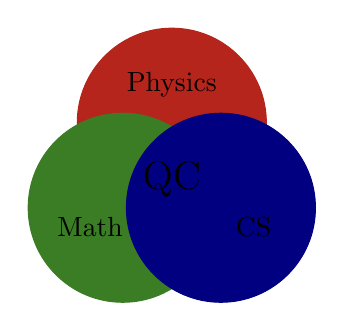
\begin{tikzpicture}[scale=0.6]
%  \begin{scope}
    \fill<1>[color=BrickRed]   ( 90:1.2) circle (2);
    \draw[color=BrickRed]   ( 90:1.2) circle (2);
    \fill<2>[color=OliveGreen] (210:1.2) circle (2);
    \draw[color=OliveGreen] (210:1.2) circle (2);
    \fill<3>[color=NavyBlue]  (330:1.2) circle (2);
    \draw[color=NavyBlue]  (330:1.2) circle (2);
%  \end{scope}
  \node<1-> at ( 90:2)    {Physics};
  \node<2-> at ( 210:2)   {Math};
  \node<3-> at ( 330:2)  {CS};
  \node<4-> [font=\Large] {QC};
\end{tikzpicture}
&
\begin{minipage}[b]{0.5\textwidth}
\begin{itemize}
    \item<1->{\textcolor<1>{BrickRed}{Physics is the study of the observable universe}}
    \item<2->{\textcolor<2>{OliveGreen}{Math is the study of logic and reasoning}}
    \item<3->{\textcolor<3>{NavyBlue}{Computer science solves problems using computation}}
\end{itemize}

\end{minipage}
\end{tabular}

\bigskip

\only<4>{

\bigskip

Quantum Computing combines all of these disciplines}
\only<1>{\ColorR{We study physics so as to understand and believe in quantum behavior}}
\only<2>{\ColorG{Quantum values and gates can be represented using linear algebra}}
\only<3>{\ColorB{Computer science lets us reason about the problems we can solve}}
\end{frame}

\begin{frame}{Prerequisites}
\begin{description}
    \item[Linear and Matrix Algebra] We use this heavily.  You must be familiar with row and column vectors, matrix multiplication, linear systems of equations.
    
    Example:  Math 309
    \item[Probability] Quantum computations are inherently probabilistic.  You need to have some background in probability, but it doesn't have to be extensive.
    
    Example:  ESE 326 or Math 3200
    \item[Circuits]  We will specify quantum computations using circuit diagrams.  Some familiarity with Boolean algebra and circuit elements depicting Boolean operations is needed.
    
    Example:  CSE 132 or CSE 260M
\end{description}
\end{frame}
\begin{frame}{Goals}
\begin{itemize}
    \item Understand and be able to construct quantum circuits to solve a problem.
    \item Sufficient background to take quantum information courses in ESE.
    \item Sufficient background to take foundational courses in Math.
\end{itemize}
\end{frame}

\section{Computation}

\begin{frame}{Computer scientists are cuckoos}{We steal ideas from other disciplines to compute things}

We can compute things using
\begin{itemize}
    \item Steam
    \item Semiconductor physics
    \item Water
    \item DNA
    \item \alert{Gravity}
    \item Quantum effects
\end{itemize}
    
\end{frame}

\begin{frame}{Using gravity to compute square roots}{We steal ideas from other disciplines to compute things}
\only<1->{How can we use gravity to compute square roots?}

\only<2-3>{We know from physics}
\only<3->{
\begin{eqnarray*}
\only<3>{\ColorR{d} & = & \frac{1}{2} a \ColorG{t}^{2} \\}
\only<4->{\ColorG{t} & = & \sqrt{\frac{2\ColorR{d}}{a}}}
\end{eqnarray*}}
\only<5->{To compute $\sqrt{n}$, we just need to drop a ball from height $\ColorR{d}=\frac{an}{2}$ and measure the time for the ball to hit the ground.}
\only<6->{

\medskip

Example:
\begin{eqnarray*}
a & = & 9.8 \mbox{ m/$s^2$} \\
n & = & 81 \\
\ColorR{d} & = & an / 2 = 369.9 \mbox{ meters}
\end{eqnarray*}
Takes 9 seconds to drop}
\end{frame}
\end{document}